\documentclass[12pt, twoside]{article}
\usepackage[francais]{babel}
\usepackage[T1]{fontenc}
\usepackage[latin1]{inputenc}
\usepackage[left=7mm, right=7mm, top=7mm, bottom=7mm]{geometry}
\usepackage{float}
\usepackage{graphicx}
\usepackage{array}
\usepackage{multirow}
\usepackage{amsmath,amssymb,mathrsfs}
\usepackage{soul}
\usepackage{textcomp}
\usepackage{eurosym}
 \usepackage{variations}
\usepackage{tabvar}


\pagestyle{empty}

\begin{document}


\section*{\center{Correction devoir maison 7}}


\subsection*{Exercice 2}

\textbf{Triangle rose:} 
Le p�rim�tre du triangle ABC est: 3,6+6+4,8=14,4m. 

L'aire de ABC est
$\dfrac{3,6 \times 4,8}{2}=8,64m^2$.


\textbf{Triangle orange:} 
Le p�rim�tre du triangle ABC est: 2,6+4+4,2=10,8cm. 

L'aire de ABC est
$\dfrac{2,4 \times 4,2}{2}=5,04cm^2$.

\textbf{Triangle vert:} 
Le p�rim�tre du triangle ABC est: 26+12,5+16,5=55dm. 

L'aire de ABC est
$\dfrac{10 \times 16,5}{2}=82,5dm^2$.

\subsection*{Exercice 3}

Pour calculer l'airedu quadrilat�re TRAP, on calcule les aires des diff�rentes
parties de la figure puis on les additionne.

Aire du triangle TPK (rectangle en K): $\dfrac{PK \times TK}{2}=\dfrac{3
\times 4}{2}=6cm^2$.


Aire du carr� TRKH: $4^2=4 \times 4=16cm^2$.

Aire du triangle RAH (rectangle en H): $\dfrac{RH \times HA}{2}=\dfrac{4
\times 5}{2}=10cm^2$.

L'aire de TRAP est donc: 10+16+9=32$cm^2$.

\subsection*{Exercice 4}


\begin{tabular}{cc}
\begin{minipage}{12cm}
\textbf{Aire de la surface des primev�res:} 


ABC est un triangle rectangle en B donc $\dfrac{4,6 \times 1,8}{2}=4,14m^2$ 

\enskip

\textbf{Aire de la surface des tulipes:} 

[EG] est la hauteur relative au c�t� [AD]. Donc
l'aire est donn�e par la formule:
 $\dfrac{EG \times AD}{2}=\dfrac{1,25
\times 1,8}{2}=1,125m^2$


\end{minipage}
&
\begin{minipage}{6cm}
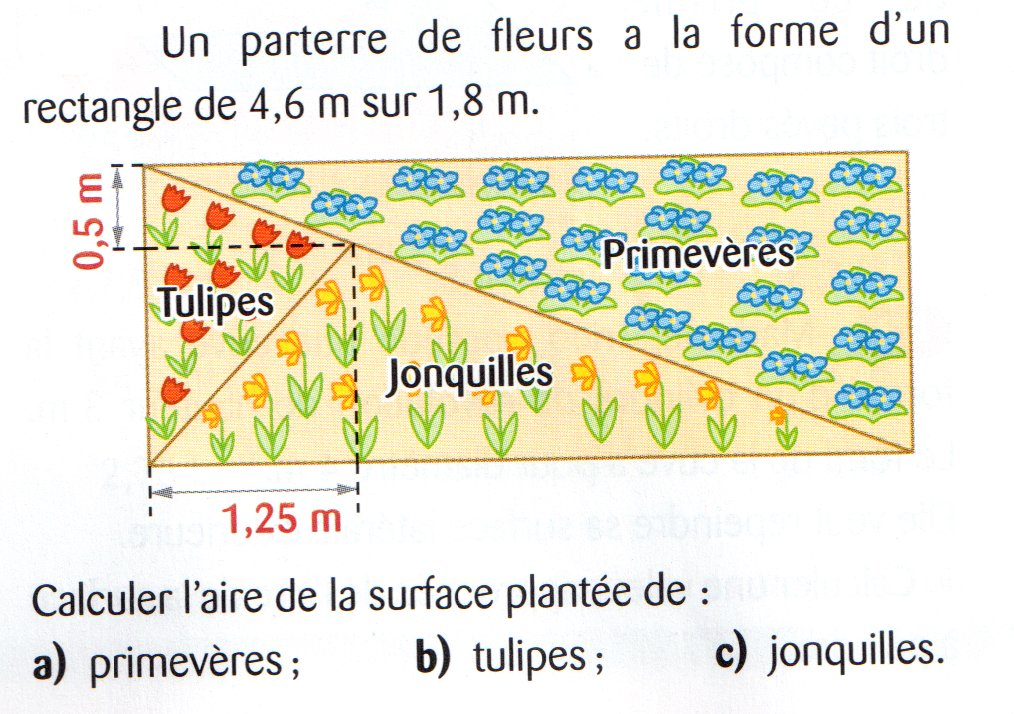
\includegraphics[width=6cm]{images/ex4.jpg}
\end{minipage}
\end{tabular}

\enskip

\textbf{Aire de la surface des jonquilles:} 

[FG] est la hauteur relative au c�t� [DC].
Donc l'aire est donn�e par la formule:

 $\dfrac{FG \times DC}{2}=\dfrac{1,3
\times 4,6}{2}=2,99m^2$ (car FG=AD-AE=1,8-0,5=1,3).


\subsection*{Exercice 5}

Notons OHS le triangle des Bermudes. Le bateau not� B est � �gale distance de
chaque lieu. Il faut donc BO=BS=BH.

On utilise la propri�t� suivante: ``Si MA=MB alors le point M est situ� sur la
m�diatrice de [AB]''.

BO=BS, on en d�duit que le point B se situe sur la m�diatrice de [OS]. 

BO=BH, on en d�duit que le point B se situe sur la m�diatrice de [OH].

BH=BS, on en d�duit que le point B se situe sur la m�diatrice de [HS]. 

Donc le point B se situe � l'intersection des trois m�diatrices du triangle
OHS: le point B est donc le centre du cercle circonscrit. Pour le placer, il
faut tracer les m�diatrices. Puis par lecture de la carte, on trouve les
coordonn�es du bateau.
\end{document}
